\documentclass[10pt]{article}

\usepackage[T1]{fontenc}
\usepackage{geometry}
\usepackage{amsmath, amssymb, amsthm}
\usepackage{bm}
\usepackage{cancel}
\usepackage{xcolor}
\usepackage{graphicx}
\usepackage{caption}
\usepackage{subcaption}
\usepackage{hyperref}
\usepackage{float}

\title{Mathematical Methods II - Assignment VII}
\author{Satvik Saha}
\date{}

\geometry{a4paper, margin=1in}
\setlength\parindent{0pt}
\renewcommand{\labelenumi}{(\alph{enumi})}
\renewcommand\CancelColor{\color{red}}
% \renewcommand\qedsymbol{$\blacksquare$}
\newcommand\ve[1]{\boldsymbol{#1}}
\newcommand\ppx[1]{\frac{\partial #1}{\partial x}}
\newcommand\ppt[1]{\frac{\partial #1}{\partial t}}
\newcommand\pp[3][]{\frac{\partial^{#1}{#2}}{\partial {#3}^{#1}}}
\newcommand\ddx[1]{\frac{d #1}{d x}}
\newcommand\ddt[1]{\frac{d #1}{d t}}
\newcommand\dd[3][]{\frac{d^{#1}{#2}}{d {#3}^{#1}}}
\newcommand\norm[1]{\left\lVert#1\right\rVert}
\newcommand\grad[1]{\ve{\nabla}#1}
\newcommand\divg[1]{\ve{\nabla}\cdot#1}
\newcommand\curl[1]{\ve{\nabla}\times#1}
\newcommand\lapl[1]{\nabla^2 #1}

\begin{document}
        \par\textbf{IISER Kolkata} \hfill \textbf{Assignment VII}
        \vspace{3pt}
        \hrule
        \vspace{3pt}
        \begin{center}
                \LARGE{\textbf{MA 2103 : Mathematical Methods II}}
        \end{center}
        \vspace{3pt}
        \hrule
        \vspace{3pt}
        Satvik Saha, \texttt{19MS154}\hfill\today
        \vspace{20pt}
        \subsection*{Fourier Series and Transforms (M.L. Boas, Chapter 7)}

        \paragraph{Section 9. Problem 2.} Write the following as the sum of an even function and an odd function.
        \begin{enumerate}
                \item $\ln|1-x|$.
                \item $(1 + x)(\sin{x} + \cos{x})$.
        \end{enumerate}

        \textit{Solution.} Given a function $f$, note that we can write it in the form
        \[
                f(x) \;=\; \underbrace{\frac{1}{2}(f(x) + f(-x))}_{g(x)} \,+\, \underbrace{\frac{1}{2}(f(x) - f(-x))}_{h(x)}.
        \]
        Note that $g$ is even and $h$ is odd, because
        \[
                g(-x) = \frac{1}{2}(f(-x) + f(x)) = g(x), \qquad h(-x) = \frac{1}{2}(f(-x) - f(x)) = -h(x).
        \]
        Thus, $f = g + h$ is the desired decomposition.
        \begin{enumerate}
                \item We write $f = g + h$, where
                \[
                        g(x) = \frac{1}{2}\ln|1 - x| + \frac{1}{2}\ln|1 + x|, \qquad h(x) = \frac{1}{2}\ln|1 - x| - \frac{1}{2}\ln|1 + x|.
                \]
                \item Again, $f = g + h$, where
                \begin{align*}
                        g(x) &= \frac{1}{2}(1 + x)(\sin{x} + \cos{x}) + \frac{1}{2}(1 - x)(-\sin{x} + \cos{x}) = \cos{x} + x\sin{x}, \\
                        h(x) &= \frac{1}{2}(1 + x)(\sin{x} + \cos{x}) - \frac{1}{2}(1 - x)(-\sin{x} + \cos{x}) = \sin{x} + x\cos{x}.
                \end{align*}
        \end{enumerate}

        \paragraph{Problem 9.} Sketch several periods of the following function (given over one period), decide whether its even or odd, and expand it
        as a Fourier series.
        \[
                f(x) = x^2, \qquad -\frac{1}{2} < x < \frac{1}{2}.
        \]

        \textit{Solution.}
        \begin{figure}[H]
                \centering        
                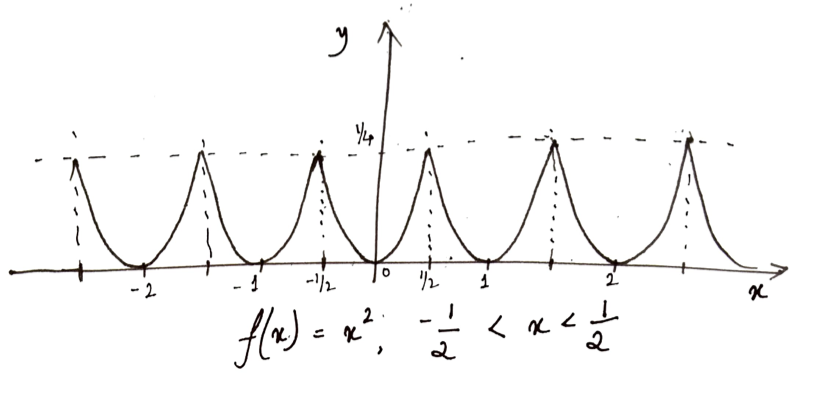
\includegraphics[scale=0.5]{./7_9.png}
        \end{figure}
        We note that the given function is even. Thus, we write
        \[
                f(x) = a_0 + \sum_{n = 1}^\infty a_n \cos{2n\pi x}.
        \]
        We calculate
        \[
                a_0 = 2\int_{0}^{\frac{1}{2}} x^2\:dx = 2\cdot \frac{1}{3}\cdot \left(\frac{1}{2}\right)^3 = \frac{1}{12}.
        \]
        For $n \geq 1$,
        \begin{align*}
                a_n = 4\int_0^1 x^2\cos{2n\pi x}\:dx 
                        &= \cancel{\frac{2}{n\pi}x^2\sin{2n\pi x}\Big|_0^{\frac{1}{2}}} - \frac{2}{n\pi}\int_0^\frac{1}{2} 2x\sin{2n\pi x}\:dx \\
                        &= \frac{1}{n^2\pi^2}x\cos{2n\pi x}\Big|_0^{\frac{1}{2}} - \frac{1}{n^2\pi^2}\cancel{\int_0^\frac{1}{2} \cos{2n\pi x}\:dx} \\
                        &= \frac{1}{n^2\pi^2}\cos{n\pi}.
        \end{align*}

        Thus,
        \[
                f(x) \;=\; \frac{1}{12} \,+\, \sum_{n = 1}^\infty \frac{1}{n^2\pi^2}\cos{n\pi}\cos{2n\pi x}.
        \]

        \paragraph{Problem 14.} Give algebraic proofs for even and odd functions that 
        \begin{enumerate}
                \item even times even = even; odd times odd = even; even times odd = odd.
                \item The derivative of an even function is odd; the derivative of an odd function is even.
        \end{enumerate}
        \textit{Solution.} Consider arbitrary even and odd functions $f_i$ and $g_i$ respectively. Thus,
        \[
                f_i(x) = f_i(-x), \qquad g_i(x) = -g_i(-x).
        \]
        \begin{enumerate}
                \item Firstly, we show that $f_1f_2$ is even.
                \[
                        (f_1f_2)(x) = f_1(x)f_2(x) = f_1(-x)f_2(-x) = (f_1f_2)(-x).
                \]
                Next, we show that $g_1g_2$ is even.
                \[
                        (g_1g_2)(x) = g_1(x)g_2(x) = (-g_1(-x))(-g_2(-x)) = (g_1g_2)(-x).
                \]
                Finally, we show that $fg$ is odd.
                \[
                        (fg)(x) = f(x)g(x) = f(-x)(-g(-x)) = -(fg)(-x).
                \]
                These establish the desired properties.

                \item Define $h\colon \mathbb{R}\to \mathbb{R}$, $x \mapsto -x$.
                Thus, the definitions of even and odd functions imply that
                \[
                        f\circ h = f, \qquad g\circ h = -g.
                \]
                Differentiating and applying the chain rule,
                \[
                        (f'\circ h)(h') = f', \qquad (g'\circ h)(h') = -g'.
                \]
                However, $h' = -1$, so
                \[
                        f'\circ h = -f', \qquad g'\circ h = g'.
                \]
                This is precisely the definition of $f'$ and $g'$ being \textit{odd} and \textit{even} respectively.
                \[
                        f'(-x) = -f'(x), \qquad g'(-x) = g(x).
                \]      
        \end{enumerate}

        \paragraph{Problem 15.} Given $f(x) = x$ for $0 < x < 1$, sketch the even function $f_c$ of period $2$ and the odd function $f_s$
        of period $2$, each of which equals $f(x)$ on $0 < x < 1$. Expand $f_c$ in a cosine series and $f_s$ in a sine series. \\

        \textit{Solution.}
        \begin{figure}[H]
                \centering        
                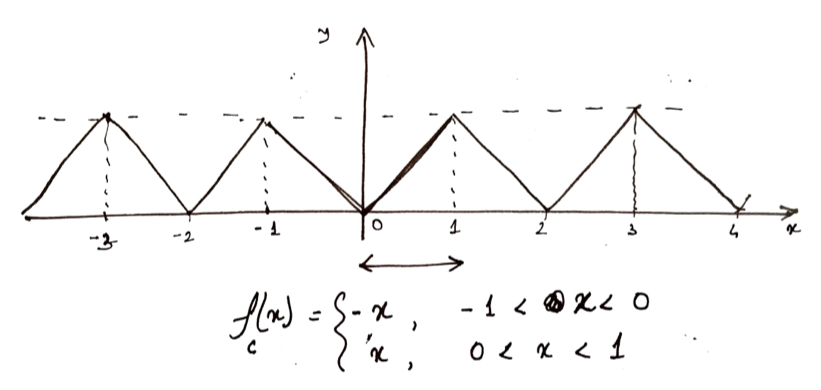
\includegraphics[scale=0.5]{./7_15_fc.png}
        \end{figure}
        \begin{figure}[H]
                \centering        
                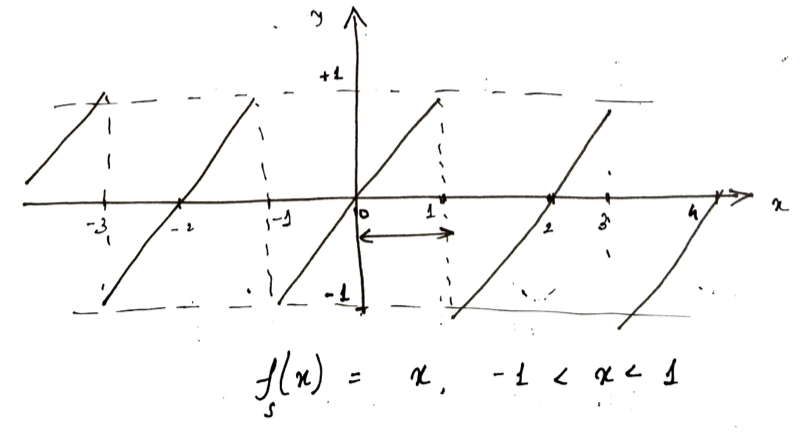
\includegraphics[scale=0.5]{./7_15_fs.png}
        \end{figure}
         We calculate the Fourier coefficients together.
        \begin{align*}
                a_0 &= \int_0^1 x\:dx = \frac{1}{2}, \\
                a_n &= 2\int_0^1 x\cos{n\pi x}\:dx = \cancel{\frac{2}{n\pi}x\sin{n\pi x}\Big|_0^1} - \frac{2}{n\pi}\int_0^1 \sin{n\pi x}\:dx
                        = \frac{2}{n^2\pi^2}(1 - \cos{n\pi}), \\
                b_n &= 2\int_0^1 x\sin{n\pi x}\:dx = -\frac{2}{n\pi}x\cos{n\pi x}\Big|_0^1 + \frac{2}{n\pi}\cancel{\int_0^1 \cos{n\pi x}\:dx}
                        = -\frac{2}{n\pi}\cos{n\pi}.
        \end{align*}
        Thus,
        \[
                f_c = \frac{1}{2} + \sum_{n = 1}^\infty \frac{2}{n^2\pi^2}(1 - \cos{n\pi})\cos{n\pi x}, \qquad
                f_s = -\sum_{n = 1}^\infty \frac{2}{n\pi}\cos{n\pi}\sin{n\pi x}.
        \]

        \paragraph{Problem 19.} Given $f(x) = |\cos{x}|$ for $0 < x < \pi$, sketch several periods of the even function $f_c$ and
        the odd function $f_s$ of periods $2\pi$ and the function $f_p$ of period $\pi$, each of which equals $f(x)$ on $0 < x < \pi$.
        Expand each of them in an appropriate Fourier series. \\

        \textit{Solution.}
        \begin{figure}[H]
                \centering        
                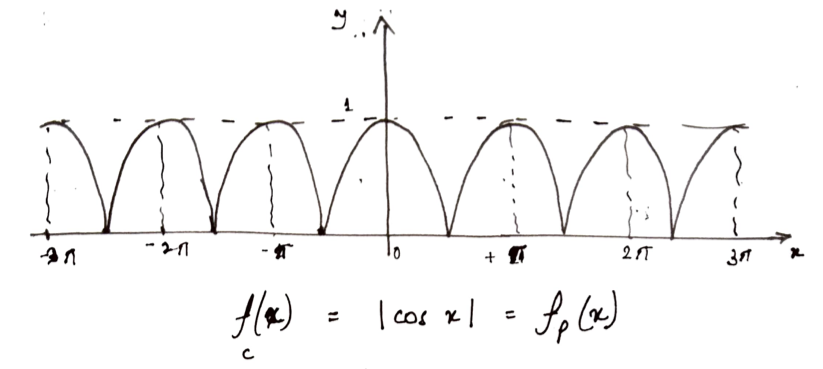
\includegraphics[scale=0.5]{./7_19_fc.png}
        \end{figure}
        \begin{figure}[H]
                \centering        
                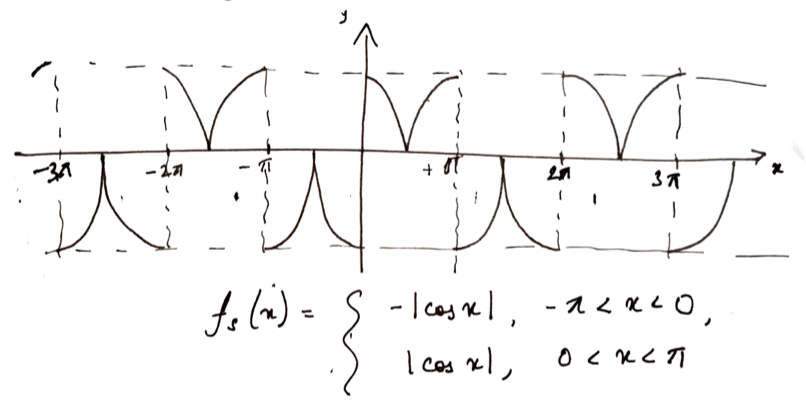
\includegraphics[scale=0.5]{./7_19_fs.png}
        \end{figure}
        Note that $f_c = f_p$. We calculate
        \begin{align*}
                a_0 &= \frac{1}{\pi}\int_0^\pi |\cos{x}|\:dx = \frac{2}{\pi}\int_0^{\pi /2}\cos{x}\:dx = \frac{2}{\pi}. \\
        \end{align*}
        When $n \neq 1$, we have
        \begin{align*}
                a_n = \frac{2}{\pi}\int_0^\pi |\cos{x}|\cos{nx}\:dx &= \frac{2}{\pi}\int_0^{\pi/2} \cos{x}\cos{nx} + \cos{x}\cos( n\pi - nx )\:dx \\
                        &= \frac{2}{\pi}\int_0^{\pi/2}\cos{x}\cos{nx} + \cos{x}\cos{nx}\cos{n\pi} + \cancel{\cos{x}\sin{nx}\sin{n\pi}}\:dx \\
                        &= \frac{2}{\pi}(1 + \cos{n\pi}) \cdot\frac{1}{2}\int_0^{\pi/2} \cos{(n + 1)x} + \cos{(n - 1)x}\:dx \\
                        &= \frac{1}{\pi}(1 + \cos{n\pi}) \left[ \frac{1}{n + 1}\sin{(n + 1)x} + 
                                \frac{1}{n - 1}\sin{(n - 1)x} \right]_0^{\pi /2}.
        \end{align*}
        Note that this vanishes when $n$ is odd. Otherwise, note that $\sin{(2n + 1)\pi /2} = (-1)^n$, so
        \[
                a_{2n} = \frac{2}{\pi}\left[\frac{1}{2n + 1}(-1)^n - \frac{1}{2n - 1}(-1)^n\right] = -\frac{4}{\pi}\cdot\frac{(-1)^n}{4n^2 - 1}.
        \]
        We can calculate $a_1$ separately. Note that the first three lines of the previous process still hold. Thus,
        \[
                a_1 = \frac{2}{\pi}(1 + \cos{\pi})\int_0^{\pi/2} \cos^2{x}\:dx = 0.
        \]
        Again, when $n \neq 1$, we have
        \begin{align*}
                b_n = \frac{2}{\pi}\int_0^\pi |\cos{x}|\sin{nx}\:dx &= \frac{2}{\pi}\int_0^{\pi/2} \cos{x}\sin{nx} + \cos{x}\sin( n\pi - nx )\:dx \\
                        &= \frac{2}{\pi}\int_0^{\pi/2}\cos{x}\sin{nx} + \cancel{\cos{x}\cos{nx}\sin{n\pi}} - \cos{x}\sin{nx}\cos{n\pi}\:dx \\
                        &= \frac{2}{\pi}(1 - \cos{n\pi}) \cdot\frac{1}{2}\int_0^{\pi/2} \sin{(n + 1)x} + \sin{(n - 1)x}\:dx \\
                        &= -\frac{1}{\pi}(1 - \cos{n\pi}) \left[ \frac{1}{n + 1}\cos{(n + 1)x} + 
                                \frac{1}{n - 1}\cos{(n - 1)x} \right]_0^{\pi /2}.
        \end{align*}
        Note that this vanishes when $n$ is even.
        Otherwise, we calculate
        \begin{align*}
                b_{4k + 1} &= -\frac{2}{\pi}\left[\frac{1}{4k + 2}(\cos{(2k + 1)\pi} - 1) + \frac{1}{4k}(\cos{2k\pi} - 1)\right] \\
                        &= \frac{2}{\pi}\cdot \frac{1}{2k + 1}, \\
                b_{4k - 1} &= -\frac{2}{\pi}\left[\frac{1}{4k}(\cos{2k\pi} - 1) + \frac{1}{4k - 2}(\cos{(2k - 1)\pi} - 1)\right] \\
                        &= \frac{2}{\pi}\cdot \frac{1}{2k - 1}.
        \end{align*}
        From the first three lines of the previous process,
        \[
                b_1 =  \frac{1}{\pi}(1 - \cos{\pi})\int_0^{\pi/2} \sin{2x}\:dx = -\frac{2}{\pi}\cdot \frac{1}{2}\cos{2x}\Big|_0^{\pi/2} = \frac{2}{\pi}.
        \]
        Thus,
        \begin{align*}
                f_c(x) = f_p(x) &= \frac{2}{\pi} - \frac{4}{\pi}\sum_{n = 1}^\infty \frac{(-1)^n}{4n^2 - 1}\cos{2nx}, \\
                f_s(x) &= \frac{2}{\pi}\sum_{n = 0}^\infty \frac{1}{2n + 1}\left[\sin{(4n + 1)x} + \sin{(4n + 3)x}\right].
        \end{align*}

        \paragraph{Problem 25.} Suppose that $f(x)$ and $f'(x)$ are both expanded as Fourier series on $(-\pi, \pi)$, with coefficients $a_n, b_n$
        and $a_n', b_n'$. Show that $b_n' = -na_n$, and obtain a simlar relation between $a_n'$ and $b_n$ using the integral definitions.
        Show that this is the same result obtained by differentiating the series term by term. \\

        \textit{Solution}. We start with the integrals
        \[
                a_n = \frac{1}{\pi}\int_{-\pi}^{+\pi} f(x)\cos{nx}\:dx, \qquad
                b_n = \frac{1}{\pi}\int_{-\pi}^{+\pi} f(x)\sin{nx}\:dx.
        \]
        We use integration by parts,
        \[
                \int u\:dv = uv - \int v\:du, \text{ or } \int uv\:dx = u\int v\:dx - \int u'\int v\:dx\:dx.
        \]
        Thus,
        \[
                a_n = +\frac{1}{n\pi}\cancel{f(x)\sin{nx}\Big|_{-\pi}^{+\pi}} - \frac{1}{n\pi}\int_{-\pi}^{+\pi}f'(x)\sin{nx}\:dx.
        \]
        \[
                b_n = -\frac{1}{n\pi}f(x)\cos{nx}\Big|_{-\pi}^{+\pi} + \frac{1}{n\pi}\int_{-\pi}^{+\pi}f'(x)\cos{nx}\:dx.
        \]
        We recognize the second terms as $-b_n' /n$ and $a_n' /n$ respectively.
        Note that the first term in the first sum vanishes because $\sin{n\pi} = 0$.
        In the second sum, we use the Dirichlet conditions and the $2\pi$ periodicity of $f$ to extrapolate its values at the points $\pm\pi$.
        \[f(-\pi) = f(+\pi) = \frac{1}{2}\left[\lim_{x \to -\pi^+} f(x) + \lim_{x \to +\pi^-} f(x)\right].\]
        This follows since the periodicty of $f$ guarantees $\lim_{x \to +\pi^+} f(x) = \lim_{x \to -\pi^+} f(x)$, and 
        $\lim_{x \to +\pi^-}f(x) = \lim_{x \to -\pi^-}$.
        Consequentially, the first term in $b_n$ also vanishes.
        Thus, multiplying by $n$, we obtain
        \[
                n a_n = -b_n', \qquad nb_n = a_n'.
        \]
        We can also see this from the Fourier series of $f$ and $f'$, assuming they both exist.
        \[
                f(x) = a_0 + \sum_{n = 1}^\infty a_n\cos{nx} + b_n\sin{nx}.
        \]
        Differentiating this once,
        \[
                f'(x) = \sum_{n = 1}^\infty -na_n\sin{nx} + nb_n\cos{nx} = a_0' + \sum_{n = 1}^\infty b_n'\sin{nx} + a_n'\cos{nx}.
        \]
        The desired relations, $b_n' = -na_n$ and $a_n' = nb_n$ follow directly from comparing terms. Note that $a_0' = 0$.

        \paragraph{Problem 26.} Find the Fourier series of the given function.
        \[
                f(x) = \begin{cases}
                        3x^2 + 2x^3, & -1 < x < 0, \\
                        3x^2 - 2x^3, & 0 < x < 1.
                \end{cases}
        \]
        Differentiate both the series and the function repeatedly until you obtain a discontinuous function. Plot these, along
        with a few terms of the corresponding Fourier series. Note the number of terms needed for a good fit. \\

        \textit{Solution.}
        Note that the given function is even. Thus,
        \begin{align*}
                a_0 &= \int_0^1 3x^2 - 2x^3\:dx = 1 - \frac{1}{2} = \frac{1}{2}, \\
                a_n = 2\int_0^1 (3x^2 - 2x^3)\cos{n\pi x}\:dx &= \frac{2}{n\pi}\cancel{(3x^2 - 2x^3)\sin{n\pi x}\Big|_0^1}
                        - \frac{2}{n\pi}\int_0^1 6(x - x^2)\sin{n\pi x}\:dx \\
                        &= \frac{12}{n^2\pi^2}\cancel{(x - x^2)\cos{n\pi x}\Big|_0^1} - \frac{12}{n^2\pi^2}\int_0^1(1 - 2x)\cos{n\pi x}\:dx \\
                        &= -\frac{12}{n^3\pi^3}\cancel{(1 - 2x)\sin{n\pi x}\Big|_0^1} + \frac{12}{n^3\pi^3}\int_0^1(-2)\sin{n\pi x}\:dx \\
                        &= -\frac{24}{n^4\pi^4}\cos{n\pi x}\Big|_0^1 \\
                        &= -\frac{24}{n^4\pi^4}(1 - \cos{n\pi}).
        \end{align*}
        Thus,
        \[
                f(x) \;=\; \frac{1}{2} \,-\, \sum_{\substack{n = 1 \\ n\text{ odd}}}^\infty \frac{48}{n^4\pi^4}\cos{n\pi x}.
        \]
        We differentiate the original function to get
        \begin{align*}
                f'(x) &= \begin{cases}
                        6(x + x^2), & -1 < x < 0, \\
                        6(x - x^2), & 0 < x < 1.
                \end{cases} \\
                f''(x) &= \begin{cases}
                        6(1 + 2x), & -1 < x < 0, \\
                        6(1 - 2x), & 0 < x < 1.
                \end{cases} \\
                f'''(x) &= \begin{cases}
                        12, & -1 < x < 0, \\
                        -12, & 0 < x < 1.
                \end{cases}
        \end{align*}
        Note that $f'''(x)$ is discontinuous. We can similarly differentiate the Fourier series
        \begin{align*}
                f'(x) &= \sum_{\substack{n = 1 \\ n\text{ odd}}}^\infty \frac{48}{n^3\pi^3} \sin{n\pi x}, \\
                f''(x) &= \sum_{\substack{n = 1 \\ n\text{ odd}}}^\infty \frac{48}{n^2\pi^2} \cos{n\pi x}, \\
                f'''(x) &= -\sum_{\substack{n = 1 \\ n\text{ odd}}}^\infty \frac{48}{n\pi} \sin{n\pi x}.
        \end{align*}

        \begin{figure}
                \centering        
                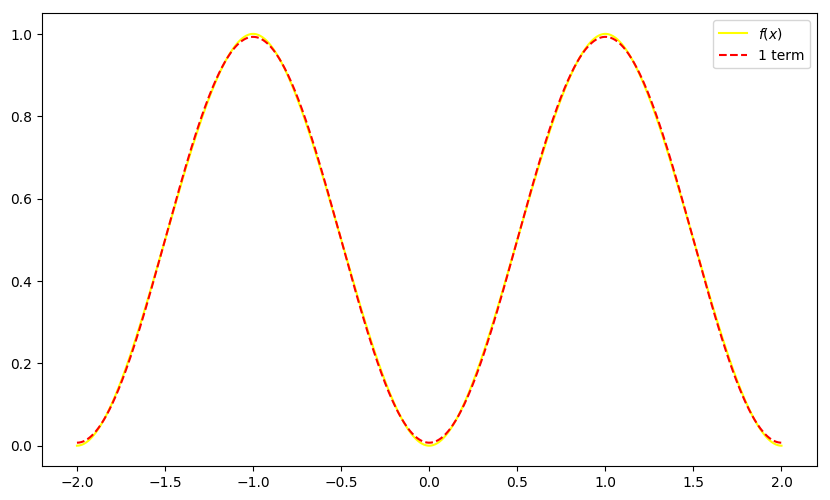
\includegraphics[width=\textwidth]{./7_f.png}
                \caption{Plot of $f(x)$. A single term of the Fourier series gives a very good fit.}              
        \end{figure}
        \begin{figure}
                \centering        
                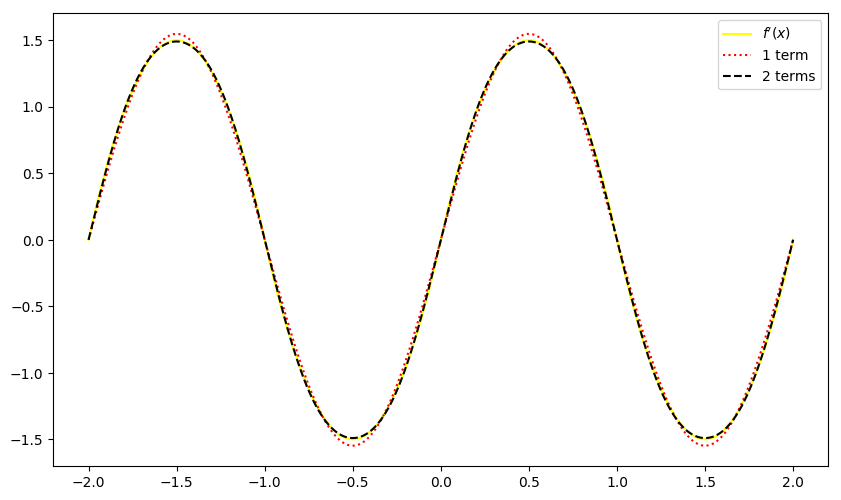
\includegraphics[width=\textwidth]{./7_f1.png}
                \caption{Plot of $f'(x)$. Two terms of the Fourier series give a good fit.}              
        \end{figure}
        \begin{figure}
                \centering        
                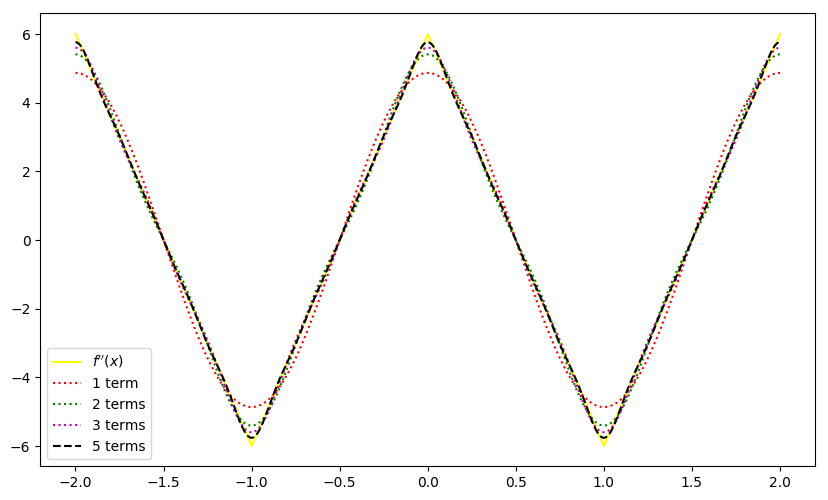
\includegraphics[width=\textwidth]{./7_f2.png}
                \caption{Plot of $f''(x)$. Five terms of the Fourier series give a good fit, although the sharp corners never fit properly.}              
        \end{figure}
        \begin{figure}
                \centering        
                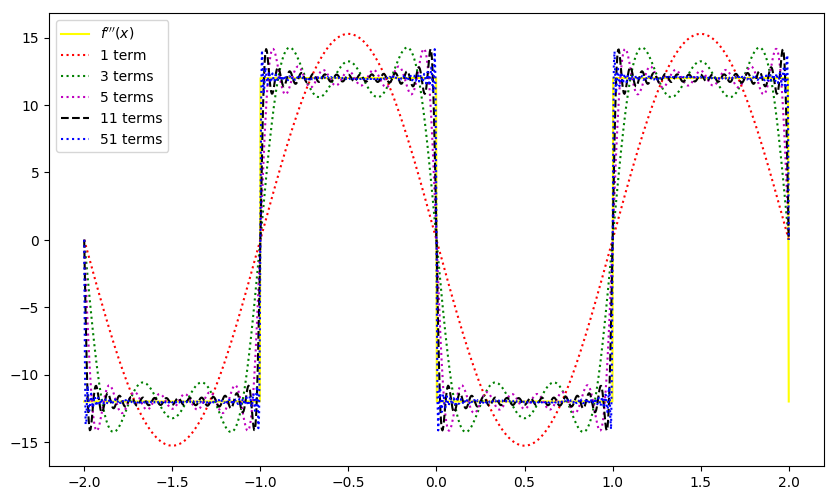
\includegraphics[width=\textwidth]{./7_f3.png}
                \caption{Plot of $f'''(x)$. Fifteen terms of the Fourier series give a good fit, although fringes always remain near the discontinuity,
                        even upon allowing around 50 terms.}              
        \end{figure}


\end{document}
